

In this chapter, we explore the social and economic mechanisms that can help in adoption and growth of community cloud model. 
We first study the social and technical context of community networks.
Next, we present first a cost-value proposition describing the conditions under which community clouds should emerge. 
Secondly, we propose a set of technical, social and economic policies that, if placed in community networks, should accelerate the uptake and help the sustainability of community clouds. 
%
Next we present a collaborative distributed architecture for community clouds, which integrates into the cloud not only the computation and storage hardware contributed to the community network by its members, but also the socio-economic contribution they make to the collective effort in the form of knowledge, time and help.
Such an architecture tailored to the specific situation and social and economic context of the community networks allows the collaborative cloud services to better fit the demands of local communities, facilitating adoption and uptake of community cloud model.


%
%% Section: INTRODUCTION
%\section{Introduction}
%\label{sec:introduction}
%
%
%% ICT has enabled collaboration and lowered costs
%Recent developments in communication technologies like Internet, email and social networking have significantly removed the barriers for communication and coordination for small to large groups bringing down the costs that obstructed collaborative production before the era of Internet~\cite{Shirky2008}.
%The ICT revolution ushered in group communication and collaborative production with popular applications now widely adopted, like social networking, social bookmarking, user-generated content, photo sharing, and many more. 
%% Community Networks
%Even infrastructures based on a cooperative model have been built, for example community wireless mesh networks gained momentum in early 2000s in response to limited options for network connectivity in rural and urban communities~\cite{Braem2013}.
%Using off-the-shelf network equipment and open unlicensed wireless spectrum, volunteers set up wireless networks in their local communities to provide network and communication infrastructure.
%These wireless networks have proved quite successful, for example
%there are several large community networks in Europe, having from 500 to 20,000 nodes, such as 
%	Athens Wireless Metropolitan Network (AWMN)~\cite{Awmn}, 
%	Freifunk~\cite{Freifunk},
%	FunkFeuer~\cite{Funkfeuer},
%	Guifi.net~\cite{Guifinet},
%	Ninux.org~\cite{Ninux},
%and many others worldwide. 
%Figure~\ref{fig:Guifi_Map_BCN_1} shows the wireless links and nodes of Guifi.net in the area around Barcelona.
%Community networks successfully operate as IP networks, since the nodes' bandwidth is shared among all the members in a reciprocal manner. 
%
%%%
%\begin{figure}[tbp]
%	\centering
%	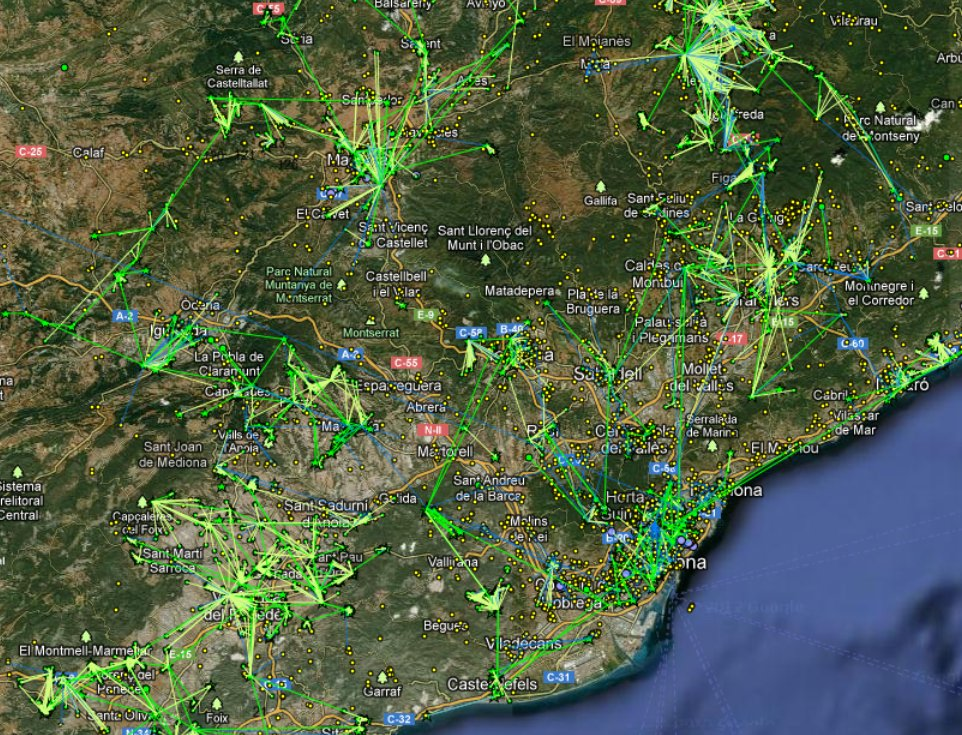
\includegraphics[width=3in,keepaspectratio]{Guifi_Map_BCN_1}
%	\caption{Guifi.net nodes and links in Barcelona}
%	\label{fig:Guifi_Map_BCN_1}
%\end{figure} 
%
%% Extending sharing in Community Networks
%Despite achieving sharing of bandwidth, community networks have not been able to extend this sharing to other computing resources like storage.
%There are not many applications and services used by members of community networks that take advantage of resources available within community networks.
%Community networks are based on voluntary contributions of participants, and economic or social incentives to encourage this have been crucial to achieve the sustainability of the community networks~\cite{Bina2006}.
%Apparently the current incentives in community networks are not sufficient enough to overcome the barriers for realising the sharing of other computing resources besides just bandwidth. 
%Applications have a challenging environment to cope with when deployed in community networks, 
%which are characterised by: 
%
%\begin{itemize}
%	\item Hardware and software diversity: The network nodes and computers are often inexpensive off-the-shelf equipment with large heterogeneity in the hardware, software and capacity. 
%	\item Decentralised Management: The network infrastructure and the computers are contributed and managed by the users. They belong to the users and are shared to build the network. There is usually no (or a rather weak) central authority that is responsible for resource provisioning.
%	\item Dynamics: The number of network and computing nodes may rapidly change when members join or leave the network, or when nodes overload or fail.
%\end{itemize}
%
%% Clouds
%Sharing of computing resources in the Internet is now commonplace because of the wide adoption of cloud computing model~\cite{Buyya2011}.
%Cloud computing provides on-demand, elastic, flexible and cost-effective access to computing resources. 
%Today's clouds are mainly provided upon a pay-per-use model, where the cloud services are offered to the consumers as a utility and by commercial providers.  
%Cloud computing allows enterprises and individuals to reduce significantly the time and capital investment in setting up their own infrastructure.
%Instead, they can request resources on demand from the cloud services providers, which not only lowers the total cost of ownership for consuming resources because of economies of scale, but leaving low level details to the service providers focus can be shifted towards building and using high level applications.
%This also applies that an individual or organisation is no longer limited by the resources present locally and owned directly. 
%When demand exceeds the current capacity, more resources can be requested on the fly from one or more cloud services providers.
%This has relevance for community networks as the members in aggregate boast much more resources than owned by a single individual or a small group.
%When members of community network can share and trade resources based on a cloud computing model, they can sell their excess capacity as the demand fluctuates and in return can take advantage of services and applications that were not possible earlier due to the limited resources locally.
%
%% Clouds in Community Networks
%The concept of community clouds has been introduced in its generic form before, e.g.~\cite{Mell2011, Marinos2009}, as a cloud deployment model in which a cloud infrastructure is built and provisioned for an exclusive use by a specific community of consumers with shared concerns and interests.
%We refer here to a specific kind of a community cloud in which sharing of computing resources is from within community networks, using the application models of cloud computing in general. 
%Members of community network can share and trade resources, they can sell their excess capacity as the demand fluctuates and in return can take advantage of services and applications that the community cloud enables, which were not possible earlier due to the limited resources on the users' local machines.
%Realising community cloud involves a lot of challenges both in technological and socio-economic context, but also promises interesting value proposition for communities in terms of local services and applications.
%
%
%Our main objective in this paper is to explore the social and economic mechanisms that can help in adoption and growth of community cloud model. 
%We contribute first a cost-value proposition describing the conditions under which community clouds should emerge. 
%Secondly, we propose a set of technical, social and economic policies that, if placed in community networks, should accelerate the uptake and help the sustainability of community clouds. 
%In our earlier work, we have explored how incentive-based resource regulation~\cite{Khan2014Prototyping, Khan2013TowardsIncentives, Buyuksahin2013} and economic policies~\cite{Khan2014Macroeconomic} can affect collaboration among the members of community networks, 
%and how the scalability issues can affect the design of a community cloud system~\cite{Khan2013Clouds}. 
%We have looked into potential distributed architecture for community cloud~\cite{Khan2014Architecture}, 
%and we are also building a prototype system to be deployed in Guifi.net community network~\cite{Jimenez2014, Jimenez2013}, 
%and investigating the performance of cloud services in these real-world settings~\cite{Selimi2014Experiences, Selimi2014TowardsApplication, Selimi2014Cloud}.
%
%The rest of the paper is organised as follows. 
%Section~\ref{sec:community-networks-scenarios} provides background to the community networks 
%and introduces possible cloud scenarios in community networks.
%Section~\ref{sec:costs-value} discusses our cost-value proposition of community clouds, and section~\ref{sec:design} proposes different mechanisms for enabling participation in community clouds.
%Section~\ref{sec:related-work} presents the related work, and  section~\ref{sec:conclusion} concludes and indicates future work.
%
